\section{Evaluation}
\label{sec:eval}
In this section, we introduce the experimental setup
and analyze the performance of different models.

\subsection{Datasets}
CNN/Daily Mail~\citep{HermannKGEKSB15}
\footnote{\url{https://cs.nyu.edu/~kcho/DMQA/}} 
is a popular summarization dataset, 
which contains news articles paired with summaries.
There are 286,817 training pairs,
13,368 validation pairs and 11,487 test pairs.
\tabref{tab:example} shows an example pair from training data.
We follow \cite{SeeLM17} in data preprocessing and use 
the non-anonymized version, which fills in the blanks with answer named entities.

Also, we tried our model on other two abstractive summarization datasets about news, which are Newsroom \citep{Newsroom18} and DUC 2002 \footnote{https://www-nlpir.nist.gov/projects/duc/guidelines/2002.html}. For Newsroom, there are 1,321,995 document-summary pairs, which are divided into training (76\%), development (8\%), test (8\%), and unreleased test (8\%). At testing, we use 8\% released test data. DUC-2002 (DUC) is a test set of document-summary pairs. We use the models trained on CNN/Daily Mail to do the test on DUC and demonstrate the generalization of the models.


\subsection{Model Parameters and Evaluation Metrics}
\label{sec:expset}
In the following experiments, 
we tokenize source documents and targets 
using the word tokenization method from NLTK (Natural Language Toolkit). 
The NLTK module is a massive toolkit, 
aimed at helping with the entire Natural Language Processing (NLP) methodology.
All the competing models contain $8$ convolutional layers in
both encoders and decoders, with kernel width of $3$.
For each convolutional layer, 
we set the hidden state size to $512$ and the embedding size to $256$.
To alleviate overfitting,
we apply a \textit{dropout} ($p=0.2$) layer to 
all convolutional and fully connected layers.
Similar to \citep{gehring2017convs2s}, we use Nesterov's
accelerated gradient method \citep{SutskeverMDH13} with gradient clipping $0.1$ \citep{PascanuMB13}, momentum $0.99$,
and initial learning rate $0.2$.
Training terminates when learning rate $\le 10e$-$5$.
Beam size $b=5$ at test time.

We set the threshold $\beta$ to $3$, 
because nearly $90\%$ 
of sections are with length$>=$3.
We set $n$ (Equation (\ref{eq:s})) to $5$,
since less than $5\%$ of reference summaries have
the LCS of less than $5$.
We use the following evaluation metrics:
\itemsep0em
\begin{itemize}

\item \textbf{ROUGE} scores (F1), including ROUGE-1 (R-1), ROUGE-2 (R-2) and
ROUGE-L(R-L)~\citep{rouge-a-package-for-automatic-evaluation-of-summaries}.
ROUGE-1 and ROUGE-2 respectively refer to the overlap of unigram (each word) and bigrams between the generated summaries and reference summaries.
ROUGE-L denotes Longest Common Subsequence (LCS) based statistics.
ROUGE-2 is the most popular metric for summarization.

\item \textbf{Repeatedness} (Rep) 
includes N-gram repeatedness, sentence repeatedness
and total repeatedness,
which reflects the effectiveness of different methods on repetition reduction.
\begin{itemize}
\item[-] \textbf{N-gram repeatedness} is the percentage of repeated N-grams 
in a summary:

\begin{equation}
Rep_{ngram} = \frac{n_{ngram}}{N_{ngram}}
\end{equation}
where $n_{ngram}$ is the number of repeated N-grams, 
$N_{ngram}$ is the total number of N-grams in a summary.
\item[-] \textbf{Sentence repeatedness} is the percentage of repeated 
sentences in a summary:
\begin{equation}
Rep_{sent} = \frac{n_{sent}}{N_{sent}}
\end{equation}
where $n_{sent}$ is the number of repeated sentences, 
$N_{sent}$ is the total number of sentences in a summary.
For sentence repeatedness, if the sentences contain the same trigram,
these sentence are repetitve sentences.
\footnote{
Any two sentences in one reference summary almost never contain 
the same trigram \citep{PaulusXS17}.}
\item[-] 
\textbf{Total repeatedness} (Algorithm \ref{alg:red}) is a comprehensive score
that unifies word-level and sentence-level repeatedness.
It is not computed by N-gram repeatedness score 
and sentence repeatedness score.

\begin{algorithm}[th]
\caption{Calculation of Total Repeatedness}
\small
\label{alg:red}
\textbf{Input}: a sentence set $s = {s_{1}, s_{2},...,s_{n}}$\\
\textbf{Output}: Total repeatedness percentage $p$
\begin{algorithmic}[1] 
\STATE Let $total$ be the sum of lengths of the sentences in $s$.
\STATE $n \leftarrow total$
\STATE $overlap \leftarrow 0$
\WHILE{$n \geq 3$}
\STATE The lengths of LCS between two sentences from $s$ comprise a length set $L$.
\STATE $n \leftarrow \max(L)$.
\STATE Find a substring $b$ with length $n$ that appears most frequently in $s$.
\STATE Let $k$ be the frequency that $b$ appears in $s$.
\STATE $overlap \leftarrow overlap + k\cdot n$
\STATE Remove every appearance of substring $b$ from sentences in $s$.
\ENDWHILE
\STATE $p \leftarrow overlap/total$
\STATE \textbf{return $p$} 
\end{algorithmic}
\end{algorithm}
\end{itemize}

\item \textbf{Repeatedness Correlation} 
measures how well 
the total repeatedness scores of summaries generated by each model
correlate with total repeatedness scores of reference summaries. 
The more correlative generated summary and reference summary are,
the better generated summary is.
The correlation is evaluated with a set of
three metrics, including Pearson correlation (r),
Spearman rank coefficient ($\rho$), and Kendall's tau coefficient ($\tau$).
Given total repeatedness scores of reference summaries (ref) and 
their corresponding generated summaries (gen),
$X=score(ref)=(x_1, x_2,..., x_n)$ and 
$Y=score(gen)=(y_1, y_2,..., y_n)$, 
we can get paired data $(X,Y)={(x_1, y_1), (x_2, y_2),..., (x_n, y_n)}$.
$n$ is the number of pairs.
\begin{itemize}	
\item[-] For Pearson correlation (r),
\begin{equation}
r = \frac{\sum_{i=1}^{n}(x_i - \overline{X})(y_i - \overline{Y})}
	{\sqrt{\sum_{i=1}^{n}(x_i - \overline{X})^{2}\cdot\sum_{i=1}^{n}(y_i - \overline{Y})^{2}}}
\end{equation}
where $\overline{X}$ and $\overline{Y}$ are the mean of variables of $X$ and $Y$.

\item[-] For Spearman rank coefficient,
\begin{equation}
\rho = \frac{\sum_{i=1}^{n}(R(x_i) - \overline{R(X)})(R(y_i) - \overline{R(Y)})}
	  {\sqrt{\sum_{i=1}^{n}(R(x_i) - \overline{R(X)})^{2}
	  \cdot\sum_{i=1}^{n}(R(y_i)-\overline{R(Y)})^{2}}}
\end{equation}
where $R(x_i)$ and $R(y_i)$ are the rank of $x_i$ and $y_i$.
$\overline{R(X)}$ and $\overline{R(Y)}$ are the mean rank of $X$ and $Y$.

\item[-] For Kendall's tau coefficient,
\begin{equation}
\tau = \frac{n_c - n_d}{n_c + n_d} = \frac{n_c - n_d}{n(n-1)/2}
\end{equation}
where $n_c$ is the number of \textit{concordant} pairs.
$n_d$ is the number of \textit{discordant} pairs.
Any pair of total repeatedness scores $(x_{i},y_{i})$ and $(x_{j},y_{j})$, where $i<j$.
They are said to be \textit{concordant},
if both $x_{i}>x_{j}$ and $y_{i}>y_{j}$; or if both $x_{i}<x_{j}$ and $y_{i}<y_{j}$.
They are said to be discordant, if $x_{i}>x_{j}$ and $y_{i}<y_{j}$; 
or if $x_{i}<x_{j}$ and $y_{i}>y_{j}$. 
If $x_{i}=x_{j}$ or $y_{i}=y_{j}$, the pair is neither concordant nor discordant.
\end{itemize}


\item \textbf{Readability} (Readable) is a human evaluation,
which can be used as the supplement to ROUGE. 
We educate human annotators to assess each summary
from four independent perspectives: 
\begin{itemize}
\item[-]
(1) Informative: How informative the summary is? 
Is the summary logically consistent with source document? 
\item[-]
(2) Coherent: How coherent (between sentences) the summary is? 
\item[-]
(3) Fluent: How grammatical the sentences of a summary are? 
\item[-]
(4) Factual: Are there any factual errors in the summary?
\end{itemize}
Readability score will be judged on the following 5-point scale:
Very Poor (1.0), Poor (2.0), Barely Acceptable (3.0), Good (4.0) and Very Good (5.0).
The score reflects the fluency and readability of the summary.
\end{itemize}

We use \textit{readability} to complement ROUGE scores 
since \cite{YaoWX17} showed that the standard 
ROUGE scores cannot capture grammatical or factual errors. 
We randomly sample 300 summaries generated by each model
and manually check their readability. 
Each summary is scored by four judges proficient in English. 
The Cohen's Kappa coefficient between them is $0.66$, 
indicating agreement. Here we use the average annotation score.

\subsection{Baselines}
Our goal is to evaluate the
effectiveness of our repetition reduction technique.
We need to select a basic model and implement different repetition reduction methods on top of it. After applying different repetition reduction methods, the basic model should be able to largely reflect the difference in the effectiveness of these repetition reduction methods. The basic model also needs to have higher training efficiency (higher speed and less memory usage) without being limited by computing resources while ensuring the quality of generation.

We choose to implement 
all existing repetition reduction techniques on top of vanilla CNN seq2seq model,
because the vanilla CNN seq2seq model is fast and enjoys the best accuracy among
the other vanilla RNN seq2seq models such as 
RNN seq2seq model and LSTM seq2seq model.~\citep{bai2018empirical,gehring2017convs2s}.
The vanilla CNN seq2seq model and vanilla self-attention-based model have similar
feature capture capabilities.
With long inputs, the self-attention-based models
will have greater computational complexity~\citep{CompareTrans}, such as Transformer. 
As the inputs of summarization are very long, the self-attention-based models
always need much more time during training and testing.
Besides, the self-attention-based models contain more training parameters,
which need more memory usage at training and testing time. 
\begin{table}[th!]
	\begin{center}
		\caption{Example of generated summaries}
		\subtable[Source document and reference summary]{
			\label{tab:a}
			\begin{tabular}{l}
				\toprule[1pt]
				\textbf{Source} \\
				\hline 
				justin timberlake and jessica biel, welcome to parenthood. \\
				the celebrity couple announced the arrival of their son, silas randall timberlake, ... \\
				the couple announced the pregnancy in january, ... it is the first baby for both .  \\
				\cmidrule[1pt]{1-1}
				\textbf{Reference} \\
				\hline 
				timberlake and jessica biel welcome son silas randall timberlake. \\
				the couple announced the pregnancy in january . \\
	    	\bottomrule[1pt]
			\end{tabular}
		}
		\qquad
		\subtable[The generated summaries of source in (a) and their ROUGE scores]{
			\label{tab:b}
			\begin{tabular}{rlc}
				\toprule[1pt] \bf model & \bf summary & \bf R-2 \\
				\cmidrule[1pt]{1-3}\textbf{COV} & \tabincell{l}{timberlake and jessica biel announced the pregnancy in january. \\
					the couple announced the pregnancy in january.} & 0.60 \\
				\hline \textbf{ATTF+SBD} & \tabincell{l}{the couple announced the arrival of their son, silas randall timberlake. \\
					the couple announced the pregnancy in january.  it is the first baby for both.} & 0.52 \\
	        	\bottomrule[1pt]
			\end{tabular}
		}
		\label{tab:compete_exp}
	\end{center}
\end{table}


We did not implement the repetition reduction methods 
on top of the seq2seq models with higher ROUGE scores,
because the effectiveness of the repetition reduction is not necessarily
reflected in the ROUGE~\citep{SeeLM17, PaulusXS17, FanGA18}.
As shown in \tabref{tab:compete_exp}, 
after reducing repetition, the summary becomes better
but the ROUGE score is not improved. 
Therefore our evaluation mainly compares
the effectiveness of different repetition reduction techniques
in terms of all four metrics above.
As known, ROUGE is not very good at evaluating abstractive summarization
and the room for improvement on the ROUGE scores are very limited.
If the repetition reduction methods 
were applied on top of the models with higher ROUGE scores, 
the differences in ROUGE scores by these repetition reduction techniques would be
indistinguishable and complicate the analysis. 
Hence, in this work, 
we construct seven baselines 
by converting
repetition reduction techniques developed on RNN seq2seq models to their
counterparts on vanilla CNN seq2seq models,
to be fair.
The baselines are as follows:
\itemsep0em
\begin{itemize}
\item \textbf{CNN} is the original convolutional seq2seq model \citep{gehring2017convs2s}. 
\item \textbf{ITA} integrates \textit{intra-temporal attention} \citep{NallapatiZSGX16} in CNN seq2seq model, which normalizes attention values using attention history through timestamps. 
\item \textbf{ITDA} adds \textit{intra-decoder attention} mechanism \citep{PaulusXS17} based on ITA,
which also normalizes attention values using past decoders states.
It is transferred to CNN seq2seq model in \citep{FanGA18}.
\item \textbf{COV} adopts the coverage mechanism \citep{SeeLM17}, where repeatedly
attending to the same locations is penalized in the form of \textit{coverage loss}. 
\item \textbf{COVP} adds the coverage penalty \citep{GehrmannDR18} to loss function,
which increases whenever the decoder repeatedly attend to the same locations of source document.
\item \textbf{SCL} adds semantic cohesion loss \citep{elikyilmazBHC18} to loss function.
Semantic cohesion loss is the cosine similarity between two consecutive sentences.
\item \textbf{DivCNN} uses Determinantal Point Processes methods(Micro DPPs and
Macro DPPs) to produce attention distribution \citep{DivC2C19}. DPPs consider both quality and diversity, which helps model attend to different subsequence in source document.
\item \textbf{TRI} uses \textit{trigram decoder} \citep{PaulusXS17} at testing. The generation of repetitive trigrams is banned during beam search.
\end{itemize}

\subsection{Results}
\label{sec:result}

\textbf{Segmentation.} As shown in \tabref{tab:punct}, we can get segments from the documents and summaries in three ways: {\em sentence-level segment}, {\em N-gram segment} and {\em punctuation-based segment}.
\begin{table}[th!]
	\begin{center}
		\caption{ROUGE scores, total repeatedness scores (\%) and Readablity scores of the summaries in CNN/Daily Mail dataset generated by the ATTF model using sentence-level, N-gram and punctuation-based segments.}
		\begin{tabular}{lccccc}
			\toprule[1pt]
			&   R-1 & R-2 & R-L & Rep & Readable \\
			\cmidrule[1pt]{1-6}
			sentence-level &  35.44 & 15.25 & 35.68 & 3.45 &3.86\\
			N-gram &  35.52 & 15.21 & 35.90 & 3.36 &3.70 \\
			punctuation-based & \bf 36.32 & \bf 15.38 &  \bf 36.09 & \bf 3.27 &\bf 4.42 \\
			\bottomrule[1pt]
		\end{tabular}
		\label{tab:seg_comp}
	\end{center}
\end{table}

 \tabref{tab:seg_comp} shows the results of ATTF trained using different segmentation methods. 
The ATTF trained by punctuation-based segments performs best in terms of all evaluation metrics. The ROUGE scores and repeatedness scores of these three segmentation methods are similar because they all redistribute the attention distribution and avoid attending to the same segments. The difference is only from the different type of segments. As shown in \tabref{tab:seg_comp}, 
the ATTF trained on sentence-level segments achieve a higher readability score than the ATTF trained on N-gram segments, and the ROUGE scores of sentence-level segmentation is lower than N-gram segmentation. The former is because N-gram segments may cause grammatical and semantic problems and the latter is because the model with sentence-level segment may lose the important information, as shown in \tabref{tab:punct}.



\textbf{Accuracy.} As shown in \tabref{tab:eval_main}, 
our model (ATTF+SBD) outperforms all the baselines in ROUGE scores, 
indicating we are able to generate more
accurate summaries. 

\begin{table}[th!]
\begin{center}
\caption{ROUGE scores on CNN/Daily Mail dataset. In our experiments, * means that the model applies the repetition reduction methods to the decoder during test.}
\subtable[The models without operations at test.]{
	    \begin{tabular}{lccc}
		\toprule[1pt]
		Model &   R-1 & R-2 & R-L \\
		\cmidrule[1pt]{1-4}
		CNN &  34.33 & 14.25 & 35.68 \\
		ITA &  34.30 & 14.20 & 35.67 \\
		ITDA & 34.62 & 14.52 &  35.94 \\
	        COV	& 35.85 & 14.81 &  35.96 \\
	        COVP & 34.53 & 14.41 &  35.81 \\
	        SCL	& 35.13 & 14.61 & 35.93 \\
	        DivCNN	& 35.64 & 15.01 & 35.84 \\
		ATTF & \bf 36.32 & \bf 15.38 & \bf 36.09 \\
		\bottomrule[1pt]
	    \end{tabular}
        }
\qquad
\subtable[The models with operations at test.]{
	    \begin{tabular}{lccc}
		\toprule[1pt]
		Model &   R-1 & R-2 & R-L \\
		\cmidrule[1pt]{1-4}
		SBD-b1* & 34.24 & 14.33 & 34.75 \\
		SBD-b2* & 35.88 & 14.83 & 35.15 \\
		SBD* & 37.19 & 15.45 & 36.03 \\
        TRI* & 36.81 & 15.47 & 36.00 \\
		ATTF+TRI* & 37.33 & 16.65 & 36.30 \\
		ATTF+SBD* & \bf 37.69 & \bf 17.02 & \bf 36.47 \\
		\bottomrule[1pt]
	    \end{tabular}
        }
\label{tab:eval_main}
\end{center}
\end{table}


Without any special operations at testing, 
our ATTF model achieves the highest score on ROUGE, showing
its effectiveness in improving summary quality.
Models with SBD or TRI at testing
are more effective than the basic CNN seq2seq model
because more information is involved in summary generation 
as a by-product of repetition reduction.
Compared with its two variants, SBD is a little slower 
but has higher ROUGE scores, reflecting its advantage due to
better choices taken globally.
Therefore, 
we use SBD as our backtracking decoder in the following experiments. 
The number of explored candidate hypotheses, up to a point of
repetition, is less than 30 tokens.
The ROUGE score of SBD is higher than TRI on R-1 and R-L, but lower on R-2. 
The reason is that R-2 and R-L respectively evaluate
bigram-overlap and longest common sequence between the reference
summary and generated summary. This is in line with different techniques 
in SBD and TRI, the former promoting the diversity of sentences and 
the latter promoting that of trigrams.
SBD has higher ROUGE scores than ATTF,
because the summaries from
SBD do not have the repetition caused by attending to similar sentences in source.
Unlike ATTF, 
SBD cannot obtain the ability to attend to different POIs through training.
In \tabref{tab:src_rep}, the sentences in SBD are not repetitive, 
but summarized from the same POI.
The summaries may lose important information when only using SBD.
The readability score of SBD is lower than ATTF in \tabref{tab:eval_repe}.

\begin{table}[th!]
	\begin{center}
		\caption{Repeatedness scores (\%) and Readability scores on CNN/Daily Mail dataset.
			The ``Gold'' denotes reference summaries, which are the most readable. By default, the readability score of reference summaries is judged to be 5.0.
		}
		\subtable[The models without operations at test.]{
			\begin{tabular}{cccccccccc}
				\toprule[1pt]
				& Gold & CNN  & ITA & ITDA & COV & COVP & SCL & DivCNN & ATTF \\
				\cmidrule[1pt]{1-10}
				1-gram & 33.79 & 56.25 & 54.44 & 51.18 & 42.18 & 52.46 & 52.23 & 38.43 & \bf 34.98 \\
				2-gram & 2.98 & 36.55 & 34.76 & 30.64 & 16.77 & 32.11 & 34.08 & 12.62 &\bf 8.16 \\
				3-gram & 0.43 & 32.62 & 31.10 & 27.14 & 12.95 & 28.59 & 30.58 & 10.15 & \bf 5.11 \\
				4-gram & 0.12 & 30.18 & 28.85 & 25.04 & 11.17 & 26.48 & 28.34 & 9.01 &\bf 4.19 \\
				Sent & 3.98 & 49.45 & 48.34 & 42.96 & 14.52 & 25.52 & 27.58 & 8.77 & \bf 6.69 \\
				\hline
				Total-Rep & 0.51 & 18.86 & 17.94 & 15.62 & 7.77 & 16.46 & 17.65 & 10.37 & \bf 3.27 \\
				\cmidrule[1pt]{1-10}
				Readable & 5.0 & 2.95 & 3.18 & 3.46 & 3.66 & 3.75 & 3.70 & 3.65 & \bf 4.42 \\
				\bottomrule[1pt]
			\end{tabular}
		}
		\qquad
		\subtable[The models with operations at test.]{
			\begin{tabular}{cccccc}
				\toprule[1pt]
				& Gold & TRI* & SBD* & ATTF+TRI* & ATTF+SBD* \\
				\cmidrule[1pt]{1-6}
				1-gram & 33.79 & 31.91 & \bf 29.88 & 32.0 & 30.83 \\
				2-gram & 2.98 & 3.17 & \bf 2.84 & 2.94 & 3.71 \\
				3-gram & 0.43 & \bf 0.0 & 0.40 & \bf 0.0 & 0.74 \\
				4-gram & 0.12 & \bf 0.0 & 0.06 & \bf 0.0 & 0.13 \\
				Sent & 3.98 & \bf 0.0 & 3.47 & \bf 0.0 & 3.44 \\
				\hline
				Total-Rep & 0.51 & \bf 0.0 & 0.44 & \bf 0.0 & 0.80 \\
				\cmidrule[1pt]{1-6}
				Readable & 5.0 & 3.62 & 3.87 & 3.75 & \bf 4.57 \\
				\bottomrule[1pt]
			\end{tabular}
		}
		\label{tab:eval_repe}
	\end{center}
\end{table}
\begin{figure}[th!]
	\centering
	\subfigure[ITA]{
		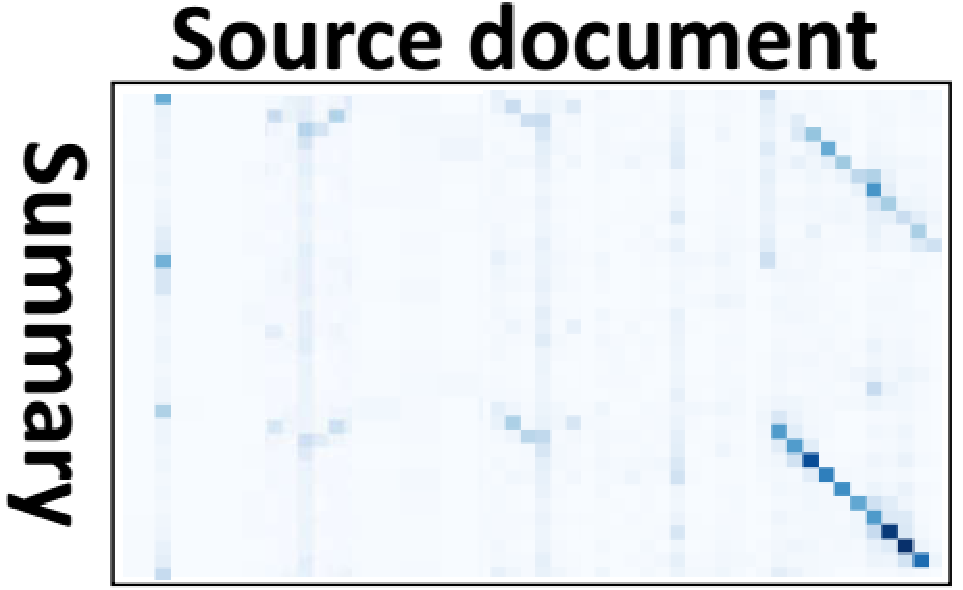
\includegraphics[width=0.26\columnwidth]{mapITA}
	}
	\quad
	\subfigure[ITDA]{
		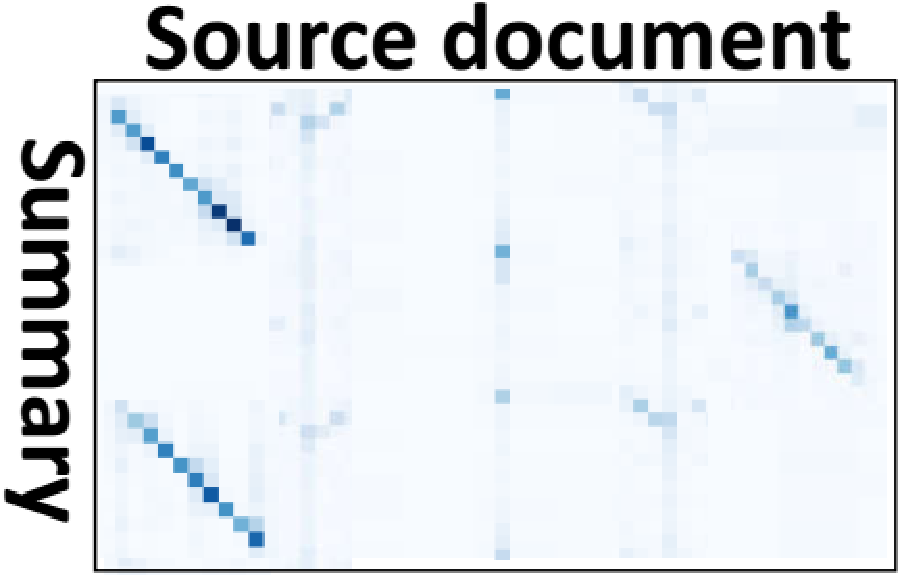
\includegraphics[width=0.26\linewidth]{mapITDA}
	}
	\quad
	\subfigure[COV]{
		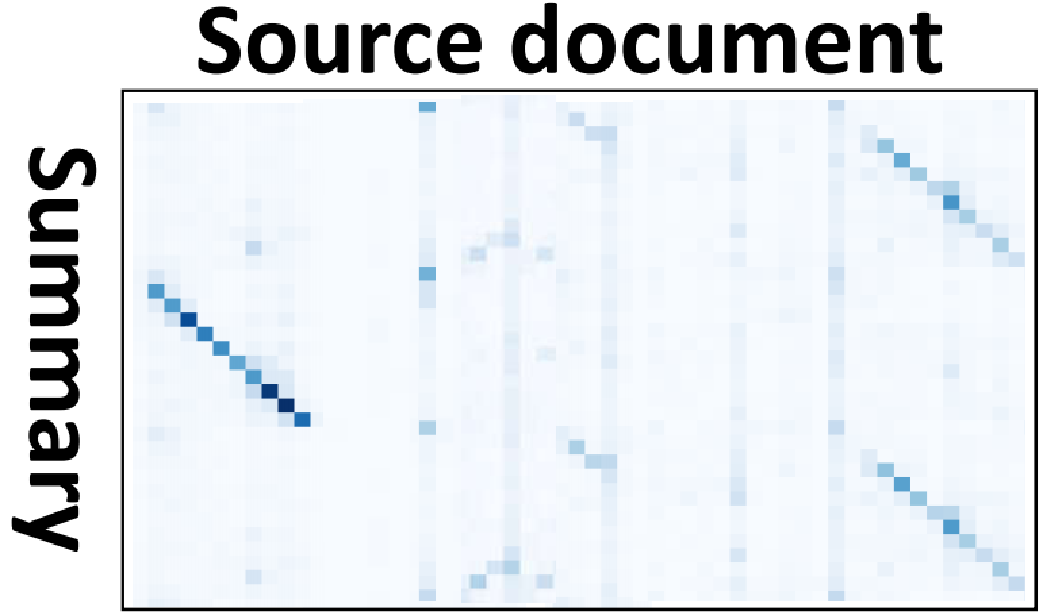
\includegraphics[width=0.26\linewidth]{mapCOV}
	}
	\quad
	\subfigure[COVP]{
		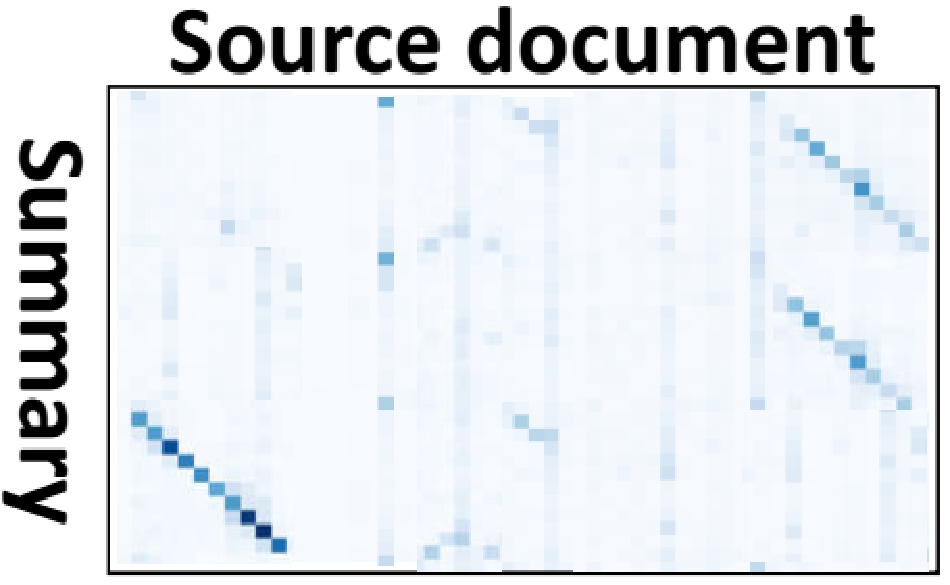
\includegraphics[width=0.26\linewidth]{mapCOVP}
	}
	\quad
	\subfigure[SCL]{
		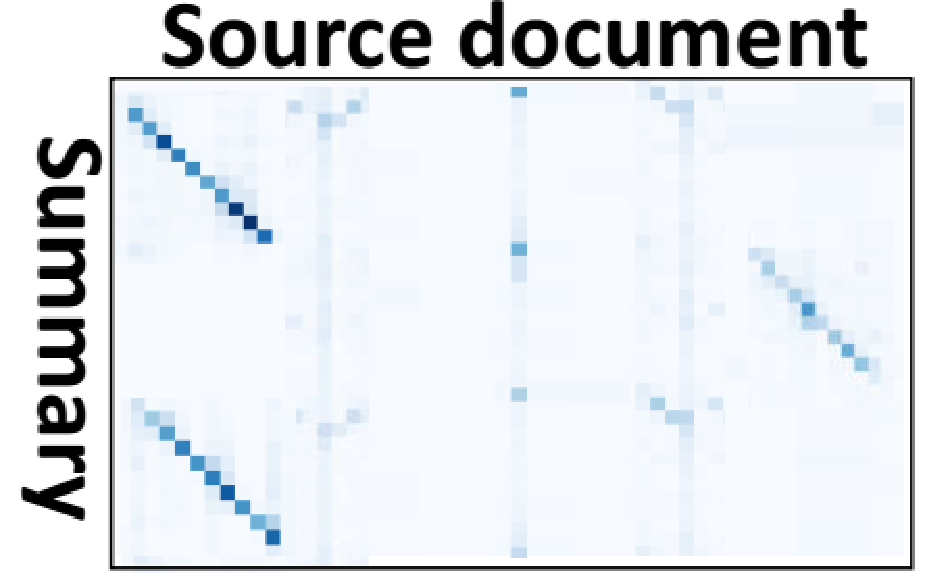
\includegraphics[width=0.26\linewidth]{mapSCL}
	}
	\quad
	\subfigure[DivCNN]{
		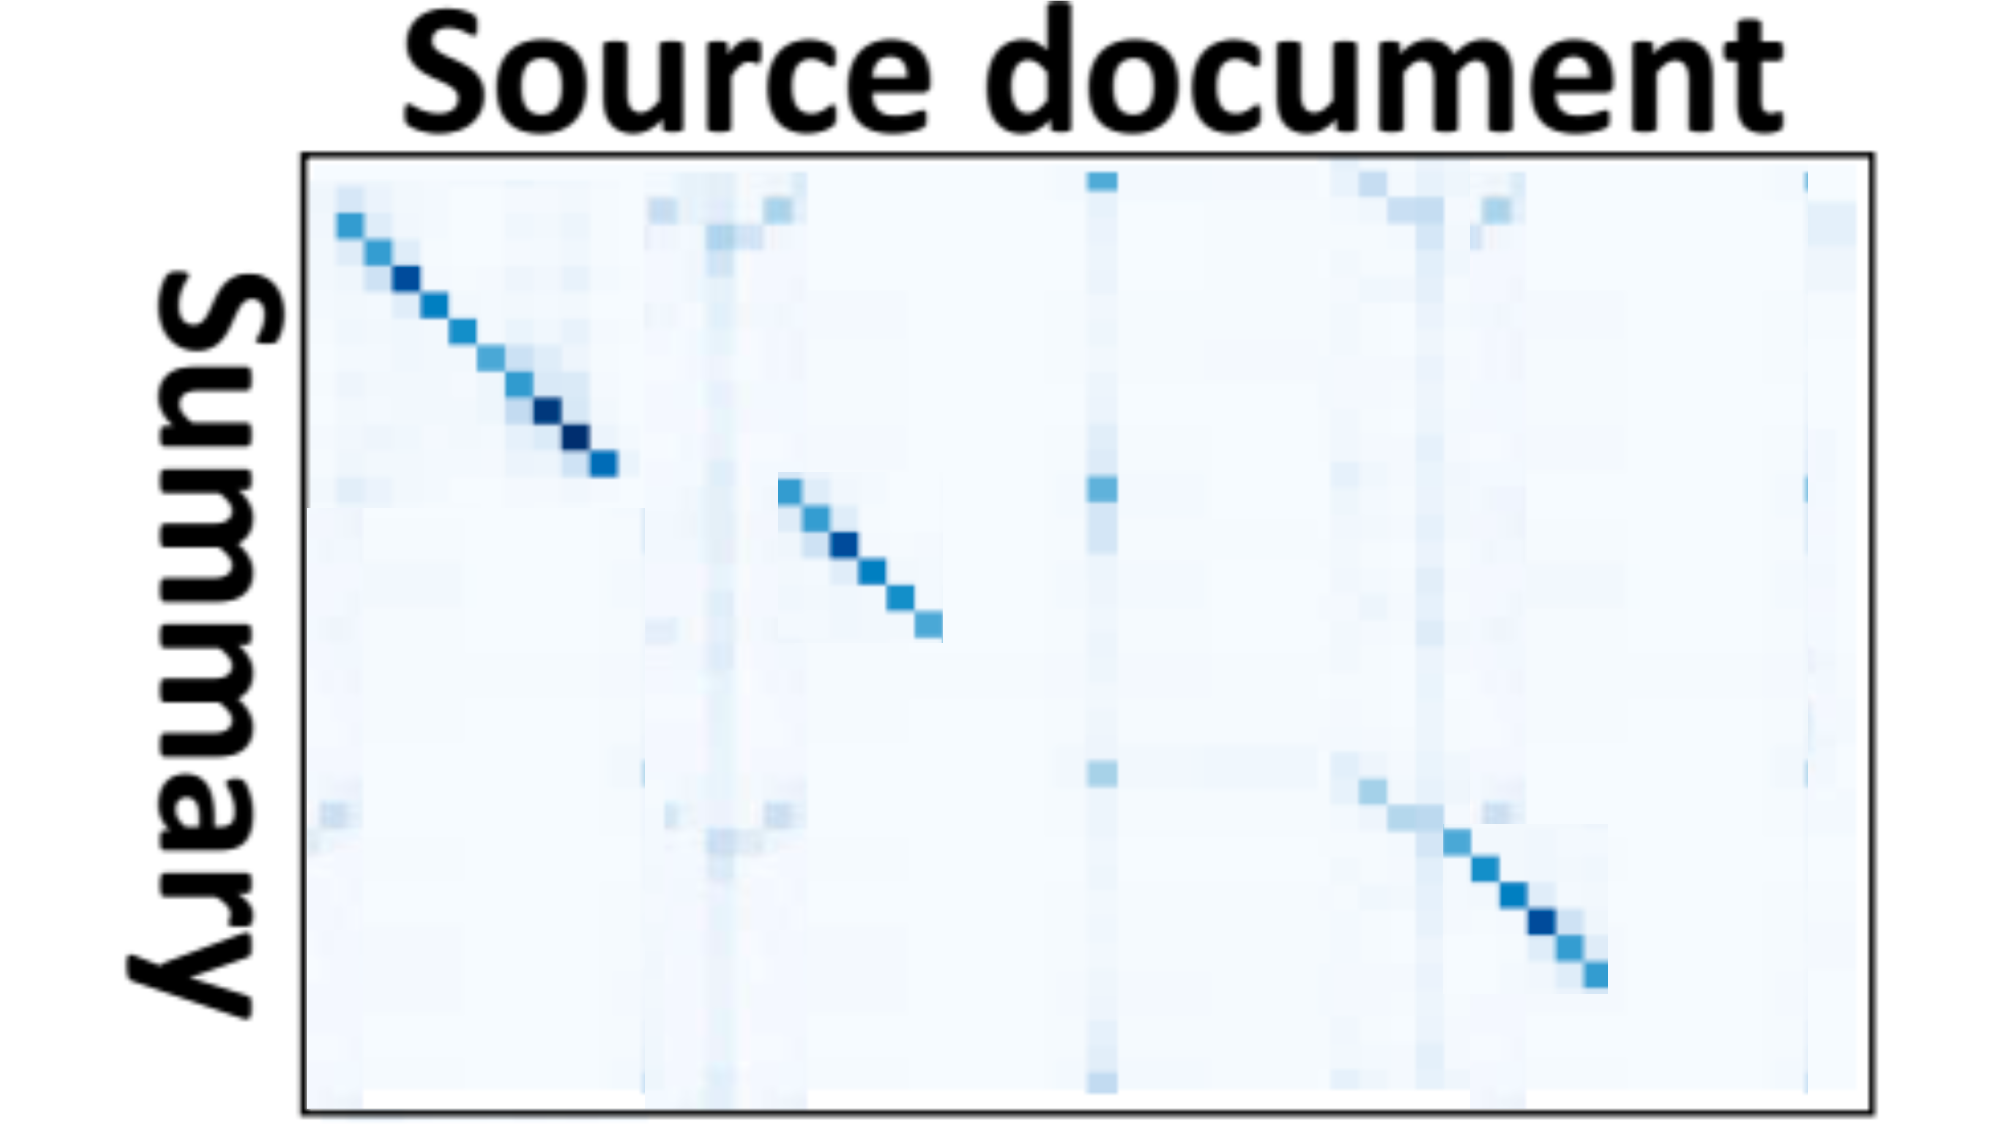
\includegraphics[width=0.26\linewidth]{mapDiv}
	}
	\quad
	\subfigure[ATTF]{
		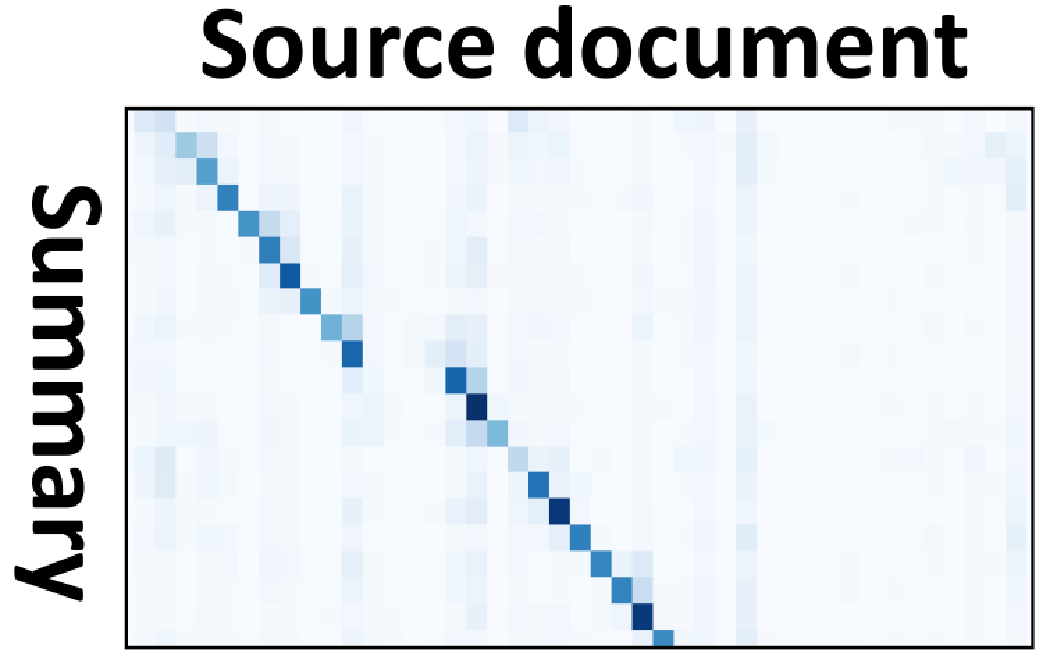
\includegraphics[width=0.26\linewidth]{map2}
	}
	\caption{Attention distribution of summaries for the source in \tabref{tab:example}}
	\label{fig:attn_maps}
\end{figure}

For models that tackle repetition both at training and test time, 
ATTF+SBD outperforms ATTF+TRI.
SBD works in synergy with ATTF, and they together process 
information with \textit{section/segment} as a unit.
ATTF+SBD scores higher ROUGE than the other baselines, 
demonstrating its power to  reduce 
repetition and generate more accurate summaries.
Besides, as shown in \tabref{tab:compete_exp}, the quality of a summary cannot be evaluated by
ROUGE scores alone.
ATTF+SBD obviously produces a better, logically more consistent summary despite 
a lower ROUGE score.  
Due to the variable nature of abstractive summarization, ROUGE is
not the optimal evaluation metric.
Repeatedness and Readability score, 
in our opinion, are important complementary metrics to ROUGE scores.  


\textbf{Repeatedness.}
To demonstrate the effectiveness of ATTF and SBD in reducing repetition, 
we compare \textit{repeatedness} (\tabref{tab:eval_repe}) 
of generated summaries.
Lower repeatedness 
means the model is more capable of reducing repetition.
In \tabref{tab:eval_repe}, Gold row shows the repeatedness scores of
reference summaries. ATTF achieves the lowest
score among all baselines without any operations at test time. 
As shown in \tabref{tab:example}, \tabref{tab:strong_methods} and \figref{fig:attn_maps},
baseline models suffer from severe repetition problem because they attend to the same POIs 
of the source document. DivCNN adjusts attention distribution in an indirect manner that adds the attention of the subsets (with high quality-diversity-score) selected from source document into the loss. Thus, DivCBNN may still attend to similar but different sentences, resulting in lower ROUGE scores and higher repeatedness. 
Besides, DivCNN is trained to attend to diversity subsets, 
which means that the selected subsets are more scattered (as shown in \figref{fig:attn_maps}) and lead to semantic incoherence.
However, ATTF attends to different POIs and generates summaries 
such as this:
\begin{itemize}
	\item[] \textbf{ATTF}: manchester city are rivalling manchester united and arsenal for defender dayot 
	pamecano. the 16-year-old joined in the january transfer window only for 
	him to opt to stay in france.
\end{itemize}

Compared with the Gold standard,
ATTF still generates some repetitive sentences,
due to similar sentences in source
such as \exref{ex:repeatsrc}.
The summary generated by ATTF and its local attention are
shown in \tabref{tab:src_rep} and \figref{fig:attn_map3}.
Also, SBD further reduces the repetition when combined with ATTF. 

\begin{table}[th!]
\begin{center}
\caption{Summaries generated from \exref{ex:repeatsrc}.}
\begin{tabular}{l}
\toprule[1pt] \textbf{Reference:} oriol romeu is on a season-long loan at stuttgart from chelsea . 
       the spanish midfielder predicts \\ the scores in saturday 's matches . oriol goes
	   head-to-head with sportsmail 's martin keown .\\
\hline \textbf{ATTF:} chelsea beat manchester united on saturday . \textit{oriol romeu is currently on a season-long loan at} \\
\textit{stuttgart .  oriol romeu is currently on a season-long loan at bundesliga side stuttgart .}\\
\hline \textbf{SBD*:} chelsea beat manchester united on saturday . chelsea face manchester 
       united in the premier league . \\ 
\hline \textbf{ATTF+SBD*:} chelsea face manchester united in the premier league on saturday . 
       oriol romeu is currently on \\ loan at stuttgart . \\
\bottomrule[1pt]
\end{tabular}
\label{tab:src_rep}
\end{center}
\end{table}

\begin{figure}[th!]
	\centering
	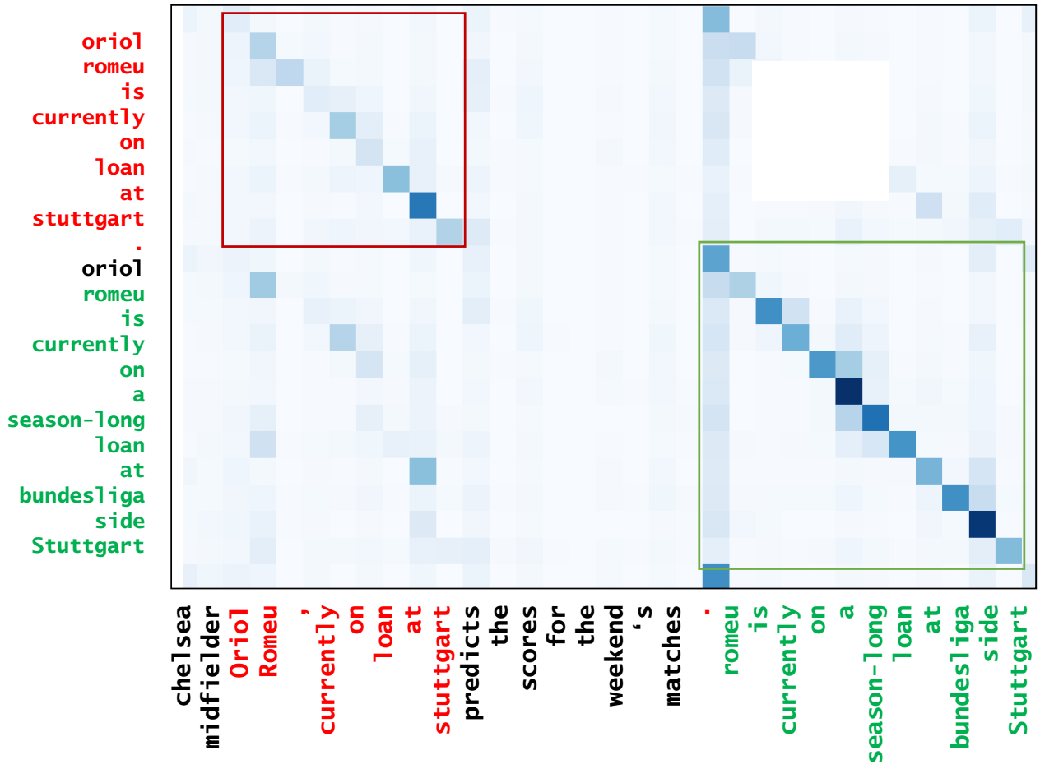
\includegraphics[width=0.78\columnwidth]{map3}
	\caption{Attention distribution for ATTF in \tabref{tab:src_rep}}
	\label{fig:attn_map3}
\end{figure}

As shown in \tabref{tab:eval_repe}, TRI has the lowest total repeatedness score.
It does not generate any repetitive N-grams (N$>$2) and sentences 
because TRI prevents the generation of the same trigrams during testing.
But as the Gold row shows, reference summaries do have some natural repetition.
Therefore we evaluate the correlation of repeatedness distribution between
generated summaries and reference summaries (\tabref{tab:eval_repcor}(a)).
Our proposed models perform best,
which indicates that ATTF and SBD are more capable of producing summaries with a natural level of repeatedness.
In addition, as shown in \tabref{tab:eval_repcor}(b), the correlations between the repeatedness and the human readability judgment are about 0.7, which means that the repeatedness score is useful. The repetition in summaries will affect coherence between sentences and the readability of summaries.

	\begin{table}[th!]
		\begin{center}
			\caption{Correlation Evaluation ($\mathbf{r}$=pearson, $\mathbf{\rho}$=spearman and $\mathbf{\tau}$= kendall's tau)}
			\subtable[Repeatedness correlation between the generated summaries and Gold summaries.]
			{
				\begin{tabular}{lccc}
					\toprule[1pt]
					& $\mathbf{r}$ & $\mathbf{\rho}$ & $\mathbf{\tau}$ \\
					\cmidrule[1pt]{1-4}
					ATTF & \bf 1.0 & \bf 1.0 & \bf 1.0 \\
					TRI* & 1.0 & 0.89 & 0.84  \\
					SBD* & \bf 1.0 & \bf 1.0 & \bf 1.0 \\
					ATTF+TRI* & 1.0 & 0.89 & 0.84 \\
					ATTF+SBD* & \bf 1.0 & \bf 1.0 & \bf 1.0 \\
					\bottomrule[1pt]
				\end{tabular}
			}
			\qquad
			\subtable[The correlation between the repeatedness of the generated summaries and the human readability judgment.]{
				\begin{tabular}{lccc}
					\toprule[1pt]
					& $\mathbf{r}$ & $\mathbf{\rho}$ & $\mathbf{\tau}$ \\
					\cmidrule[1pt]{1-4}
					ATTF & 0.78 & 0.74 & 0.70 \\
					SBD* & 0.75 & 0.71 & 0.68 \\
					ATTF+SBD* & 0.75 & 0.74 & 0.69 \\
					\bottomrule[1pt]
				\end{tabular}
			}
			\label{tab:eval_repcor}
		\end{center}
	\end{table}
\textbf{Readability.}
As shown in \tabref{tab:eval_repe}, 
the models with ATTF achieve the
highest readability score among all baselines, 
which means ATTF is more readable.
As shown in \tabref{tab:eval_repe}(b),
TRI achieves the best scores on repeatedness, 
but lower readability scores than other models.
Readability is a human evaluation metric considering the logical correctness.
(See \secref{sec:expset}). 
As shown in \tabref{tab:eval_repe} and \tabref{tab:generalization}, the Readable scores of the models with TRI are lower than the models with SBD, which indicates the effectiveness of SBD on logical correctness. Specially, after using TRI, the readability of ATTF+TRI becomes lower than ATTF. 
This means that the TRI will bring logical incorrectness
 to the generated summaries.
TRI interrupts the process of sentence generation during beam search through trigrams that cannot reflect the complete grammatical structure and semantic information. 
TRI is likely to generate summaries with more grammatical and factual errors. 
SBD forbids the repetition at sentence-level during testing, which considers complete grammatical structure and semantic information.
As shown in \tabref{tab:strong_methods} and \tabref{tab:sbd_exp}, SBD weakens the influence of the meddling of sentence generation during beam search
and generates more readable summaries.
The higher ROUGE scores show that SBD enhances the performance of CNN and ATTF by reducing the repetitive unreadable sentences. 




\textbf{Speed.} 
We compare the speed of our model on CNN/Daily Mail to RNN~\citep{SeeLM17}, FastRNN~\citep{P18-1063} and Transformer-large~\citep{Attn17}
which used K40. 
We perform experiments on GTX-1080ti and scale the speed 
reported for the RNN methods,
since GTX-1080ti is twice as fast as K40~\citep{gehring2017convs2s}. 
\begin{table}[th!]
	\centering
	\caption{Time and speed of training and testing. The training time of the model with SBDs
		is empty because SBDs are only used during testing.}
	\begin{tabular}{lcccc}
		\toprule[1pt]
		\multirow{2}{*}{Model} & Train & \multicolumn{3}{c}{Test} \\
		\cmidrule[1pt](lr){2-2}\cmidrule[1pt]{3-5}
		& Time (h) & Time (s) & summaries/s & tokens/s \\
		\cmidrule[1pt]{1-5}
		RNN  & 336.54 &21600 & 0.48 & 29.60 \\
		FastRNN & 98.4  & 3600 & 2.92 & 219.60 \\
		Transformer & 115.44 & 2094.6 & 5.65 & 214.83 \\
		\hline
		CNN & 48.3 &346.1 & 30.36 & 1343.46 \\
		SBD-b1* & - & 412.8 & 25.46 & 1126.38 \\
		SBD-b2* & -  &843.5 &12.16 & 551.24 \\
		SBD* & - &912.8 & 11.51 & 493.68 \\
		ATTF & 108 &1332 & 7.89 &  349.00 \\
		ATTF+SBD* & - &1832.3 & 5.74 &  253.77 \\
		\bottomrule[1pt]
	\end{tabular}
	\label{tab:eval_speed}
\end{table}

As shown in \tabref{tab:eval_speed}, the CNN is faster than Transformer based on multi-head self-attention mechanism.
In terms of computational complexity,
\cite{Attn17} show that the per-layer complexity of self-attention is $O(n^2d)$ and the per-layer complexity of CNN is $O(knd^2)$. $n$ is the sequence length, $d$ is the representation dimension and $k$ is the kernel width of convolutions.  So the difference between the complexity of Transformer and CNN depends on $n$, $d$ and $k$. 
In our experiments, we follow~\cite{gehring2017convs2s} in the experimental setting for CNN and \cite{Attn17} for Transformer. Both experimental settings are standard settings of the vanilla models. 
As the average sequence length of source documents in our datasets is more than $500$, the $n$ in the complexity of CNN and Transformer is greater than $500$. 
The representation dimension of CNN, $d_{cnn}$, is $256$.  
The representation dimension of Transformer, $d_{trans}$, is $1024$.
The kernel width of CNN is $3$. 
Thus, in our experiment, the speed of CNN is faster. 
The training speed and testing speed of CNN+ATTF 
are faster than RNN seq2seq model and Transformer
since the training of CNN is parallel.
The gap of training/testing time between ATTF and Transformer is not much larger,
but the memory usage of Transformer is much larger than ATTF.
This is because that Transformer has more trainable parameters than ATTF.
The training speed and testing speed of FastRNN are faster than RNN
because FastRNN is not an end-to-end model. FastRNN is a two-stage framework, which first uses an extractor to extract several salient sentences from source document and then uses an abstractor to summarize each salient sentence. The final summary is the concatenation of these summarized salient sentences. The extractor in FastRNN is a pointer network with a sequence of sentences as input.
The encoder of extractor is the same as RNN. The FastRNN adopts RNN as abstractor and trains extractor and abstractor in parallel, which speeds up the encoder and decoder of RNN seq2seq model by shortening the input and output. As an end-to-end model, the input and output of our CNN+ATTF model are sequences of words in complete source document and summary, which are much longer than the input and output of the extractor and abstractor of FastRNN. The training speed of CNN+ATTF is similar to FastRNN as the CNN can be trained in parallel. The testing speed of CNN+ATTF is faster than FastRNN because FastRNN should extract sentences first and then abstract each sentence during test.


The convergence rate of models with ATTF depends on three aspects:
{\em dataset}, {\em basic model} and {\em experimental settings}.
For {\em dataset}, ATTF redistributes the attention distribution between source documents and summaries during decoding,
which dynamically searches the attended segment in source by the predicted segments in summary.
Thus, the convergence rate of the models with ATTF depends on the length of source documents and summaries.
The ATTF applied on better {\em basic models} converges faster,
because better basic models learn the alignment between source documents and summaries better.
The {\em experimental setting} also impacts the convergence rate of the model with ATTF.
At the beginning of training, a large learning rate makes the model converge faster. 
When most of the samples have been trained, 
the model converges rapidly by decreasing the learning rate.

As shown in \tabref{tab:eval_main} and \tabref{tab:eval_speed}, 
SBD is the best sentence-level backtracking decoder.
Compared with SBD-b1 and SBD-b2,
SBD logs higher ROUGE scores without losing much on speed. 
ATTF+SBD achieves the best ROUGE scores 
and its training time and testing time do not increase too much.



\textbf{Generalization.} 
\tabref{tab:generalization} shows the generalization of our abstractive system to other two datasets, Newsroom and DUC 2002, where our
proposed models achieve better scores than vanilla CNN seq2seq model in terms of ROUGE scores, readability and repeatedness. 
We use the same settings of $\beta=3$ in \secref{sec:des} and $n=5$ in Equation \eqref{eq:s}, because the proportion of segments with length greater than 3 and reference summaries with LCS greater than 5 were about 90\%. As shown in \tabref{tab:generalization}, our proposed models can generalize better on other datasets about news, along with repetition reduction and the improvement of readability.
This shows that our proposed models can be generalized well.
\begin{table}[th!]
	\begin{center}
		\caption{ROUGE scores, total repeatedness (Rep) and readability on Newsroom and DUC}
		\begin{tabular}{lcccccccccc}
			\toprule[1pt]
			\multirow{2}{*}{Model} & \multicolumn{5}{c}{Newsroom} &\multicolumn{5}{c}{DUC} \\
			\cmidrule[1pt](lr){2-6} \cmidrule[1pt]{7-11}
			&R-1 & R-2 & R-L& Rep & Readable &R-1 & R-2 & R-L & Rep & Readable\\
			\cmidrule[1pt]{1-11}
			CNN &  27.43 & 18.62 & 26.77 & 20.38 & 2.65 & 26.02 & 8.76 & 21.05& 19.32 & 2.32 \\
			TRI* &  27.96 & 19. 83 & 27.01 & \bf 0.0 & 2.84 & 26.75 & 9.34 & 22.19& \bf 0.0 & 2.51 \\
            SBD* &  28.20 & 20.17 & 26.94 & 0.62 & 3.02 & 26.86 & 9.27 & 22.75& 0.43 & 2.85 \\
            ATTF &  28.43 & 20.05 & 27.32 & 1.53 & 3.42 & 26.94 & 9.50 & 22.33& 1.72 & 3.11 \\
			ATTF+SBD* &  \bf 28.93& \bf 21.46 & \bf 27.55 & 0.58 & \bf 3.73 & \bf 27.02 & \bf 9.56 & \bf 23.05& 0.40 & \bf 3.5 \\
			\bottomrule[1pt]
		\end{tabular}
		\label{tab:generalization}
	\end{center}
\end{table}

\textbf{Normalization.} The attention scores of the basic attention mechanism without filtering satisfy the probability distribution. 
As for the filtered attention scores of ATTF, we penalize the attention scores of the tokens that have been attended to in the source document and keep the attention scores of other tokens in the source document the same. In this way, we can keep the difference of attention scores between the tokens that have not been attended to, which may avoid ignoring some source contents that need to be summarized.
After re-normalizing the filtered attention scores, 
the decoder tends to attend to the tokens of the source document with high filtered attention scores. It can also prevent the attention scores of the tokens that have not been attended to from too small.

\begin{table}[th!]
	\begin{center}
		\caption{The comparison of ATTF and the re-normalized ATTF (Norm ATTF).}
		\subtable[The recall, precision and F1 score of R-2.]
		{
			\begin{tabular}{lccccccccc}
				\toprule[1pt]
				\multirow{2}{*}{Model} & \multicolumn{3}{c}{CNN/Daily Mail} & \multicolumn{3}{c}{Newsroom} &\multicolumn{3}{c}{DUC} \\
				\cmidrule[1pt](lr){2-4}\cmidrule[1pt](lr){5-7}\cmidrule[1pt](lr){8-10}
				&Precision & Recall & F1 & Precision & Recall & F1 & Precision & Recall & F1 \\
				\cmidrule[1pt]{1-10}
				ATTF & 14.71 & 16.65 & 15.38& 19.23& 23.82 & 20.05 & 7.88 &11.48 & 9.50 \\
				Norm ATTF &  16.18 & 14.47 & 15.32 & 22.94 & 19.44 & 19.97 & 9.82 & 9.07 & 9.54 \\
				\bottomrule[1pt]
			\end{tabular}
		}
		\qquad
		\subtable[The example of generated summaries.]{
			\begin{tabular}{ll}
				\toprule[1.2pt]
				\multicolumn{2}{l}{\bf Source document} \\
				\hline
				\multicolumn{2}{l}{\tabincell{l}{......police have been left stunned after coming across a car parked on a busy street covered in hundreds of  \\ chili peppers . \underline{traffic and highway patrol command shared the bizarre image on their facebook page} , showing\\ a silver car on the side of the road laden down with a vast amount of large red chillies . according to several \\ commenters on the post , the incident occurred on bridge st in hornsby on the upper north shore of sydney \\ and \underline{is a regular occurrence}......}} 
				\vspace*{0.5mm}\\
				\cmidrule[1.2pt]{1-2} 
				\multicolumn{2}{l}{\bf Reference summary} \\
				\hline
				\multicolumn{2}{l}{\tabincell{l}{police have come across a car covered in chili peppers . the car was parked on the side of a busy street in\\ hornsby . according to facebook users , it is a regular occurance .}}\\
				\cmidrule[1.2pt]{1-2} 			
				ATTF &  \tabincell{l}{police have come across a car parked on a busy street covered in hundreds of chili peppers . \\ \underline{traffic and highway patrol command shared the image on their facebook page.} \\ The incident occurred on bridge st in hornsby and \underline{is a regular occurrence.}\vspace*{0.5mm} } \\
				\hline
				Norm ATTF & \tabincell{l}{police have come across a car parked on a busy street covered in hundreds of chili peppers . \\ The incident occurred on bridge st in hornsby .} \\
				\bottomrule[1.2pt]
			\end{tabular}
		}
		\label{tab:norm}
	\end{center}
\end{table}


As shown in \tabref{tab:norm}, the R-2 F1 scores of ATTF and ATTF with re-normalized attention scores (Norm ATTF) are similar over all datasets. 
ROUGE recall measures how well a generated summary matches
its corresponding reference summary by counting the percentage of matched n-grams in the reference.
ROUGE precision 
indicates the percentage of n-grams in the generated summary overlapping with the reference.
ATTF is always better than Norm ATTF on R-2 recall,
and Norm ATTF is better than ATTF on R-2 precision.
As shown in \tabref{tab:norm}(b), since the difference of attention scores is not magnified by normalization, 
the summary generated by ATTF can more comprehensively attend to the information in the source. 
However, when the attention scores of the tokens that have not been attended to are too small, the decoder may attend to less important information of the source, 
such as ``traffic and highway patrol......'' (ATTF row) in \tabref{tab:norm}(b).
The summary generated by Norm ATTF is likely to miss some important information,
such as ``it is a regular occurrence.'',
due to the magnified differences between filtered attention scores.

\textbf{Comparison of ATTF and TRI.} In our experiments, 
the TRI is the basic CNN seq2seq model with trigram decoder during test.
For ROUGE scores, as shown in \tabref{tab:eval_main} and \tabref{tab:generalization},
ATTF gets lower ROUGE scores than TRI on CNN/Daily Mail and higher ROUGE scores on Newsroom and DUC. 
For repeatedness scores, as shown in \tabref{tab:eval_repe} and \tabref{tab:generalization}, the difference between ATTF and TRI in Newsroon is smaller than that between ATTF and TRI in CNN/Daily Mail.
As some of the source documents in CNN/Daily Mail have the similar but different segments (as shown in \figref{fig:attn_map3}), 
ATTF may attend to such segments and generate summaries with repetition.
The summaries with repetition always achieve lower ROUGE scores.
The better performance of ATTF on Newsroom and DUC 
indicates the ATTF is more effective than TRI in the case of the datasets without repetition in source document.
As shown in \tabref{tab:eval_repcor}, the repeatedness correlation scores of ATTF are higher than TRI, which indicates the summaries generated by ATTF are more similar to human-written summaries.
Besides, the readability scores of ATTF are better than TRI on all datasets,
which means that the summaries generated by the attention-based modification 
are more fluent and readable than simple trigram blocking.


\textbf{Significance Test.} We use significance test to prove that the ROUGE scores in \tabref{tab:eval_main} are reliable.
We take t-test 
\citep{loukina2014automatic}
as our significance test to
measure that the ROUGE scores between our proposed approach (ATTF+SBD) and each baseline are significant or not. 
As shown in \tabref{tab:ttest},
all p-values are less than 0.05. 
The smaller p-value, the higher significance.
Thus, the difference in the similarity results is significant. 

\begin{table}[th!]
	\begin{center}
		\caption{p-value of significance test between 
			our best proposed model (ATTF+SBD) and baselines on ROUGE scores}
		\begin{tabular}{lcccccccc}
			\toprule[1pt]
			Model & CNN & ITA & ITDA & COV & COVP & SCL & DivCNN & TRI \\
			\cmidrule[1pt]{1-9}
			R-1 &  2.32e-35 & 6.14e-34 & 2.76e-32 & 4.14e-30 &2.51e-32 &3.11e-32 & 2.28e-31 & 5.25e-30\\
			R-2 &  6.34e-48 & 2.12e-48& 4.52e-44 & 4.61e-50& 3.17e-41& 3.29e-44 &4.27e-40 &1.33e-43\\
			R-L & 3.68e-10 & 5.67e-12 & 3.94e-12 & 7.12e-12&2.15e-10 & 3.43e-15&6.81e-10&3.67e-12\\
			\bottomrule[1pt]
		\end{tabular}
		\label{tab:ttest}
	\end{center}
\end{table}

Overall, the summaries generated by sequence-to-sequence models with attention mechanism always contain repetition.  
Through our observations, there are two reasons for repetition in abstractive summarization.
One is that the traditional attention mechanisms attend to the same location in source document at decoding.
The other is that the attention mechanism attends to the repetitive sentences in different locations in source document. 
As shown in \figref{fig:attn_maps} and \tabref{tab:src_rep},
our proposed ATTF and SBD effectively mitigate the above two problems.  
As ATTF deals with incorrect attention distribution
between the inputs of encoder and decoder to 
reduce repetition in generated summaries,
the seq2seq models with attention mechanism between encoder and decoder
can be improved via ATTF.
The SBD can only be used at testing, which is suitable for the models with decoder.
Since RNN-based and transformer-based seq2seq models,
including attention mechanism between encoder and decoder,
always suffer from repetition in generated summaries, 
we can reasonably deduce that these models will benefit from our proposed ATTF and SBD as well.
The higher ROUGE scores (\tabref{tab:eval_main}) of our model mean that
the summaries generated by our model are more similar to their corresponding reference summaries.
The natural-level repeatedness and higher readability score (\tabref{tab:eval_repe}) of our model indicate 
that our model can produce summaries with higher quality.
ATTF is applied to the attention mechanism between encoder and decoder,
which impacts the time of decoding at training and testing.
SBD only impacts the time of decoding during test.
ATTF+SBD takes about the same amount of time for additional models to slow down.
For RNNs and transformers, after adding ATTF+SBD,
there would be less than 6 times slowdown
(As shown in Table 11, for the vanilla CNN, there is a roughly 6 times slowdown after adding ATTF+SBD.)
since RNNs and transformers spend more training time and testing time on encoding than CNN.
As a result, our model can improve the reading speed and accuracy of reading comprehension.


